\chapter{Neural networks}


%====================================================================================================
\section{History}

%----------------------------------------------------------------------------------------------------
\subsection{Biological inspiration}
Artificial neural networks were originaly created as a way of modeling behavior of biological
neurons.
Neurons are at their core cells so most of metabolic processes common for animal cells also
occur in them. However just like red blood cells neural cells do not divide on their own and new
neurons are generated by specialised stem cells.
\begin{figure}[hb]
	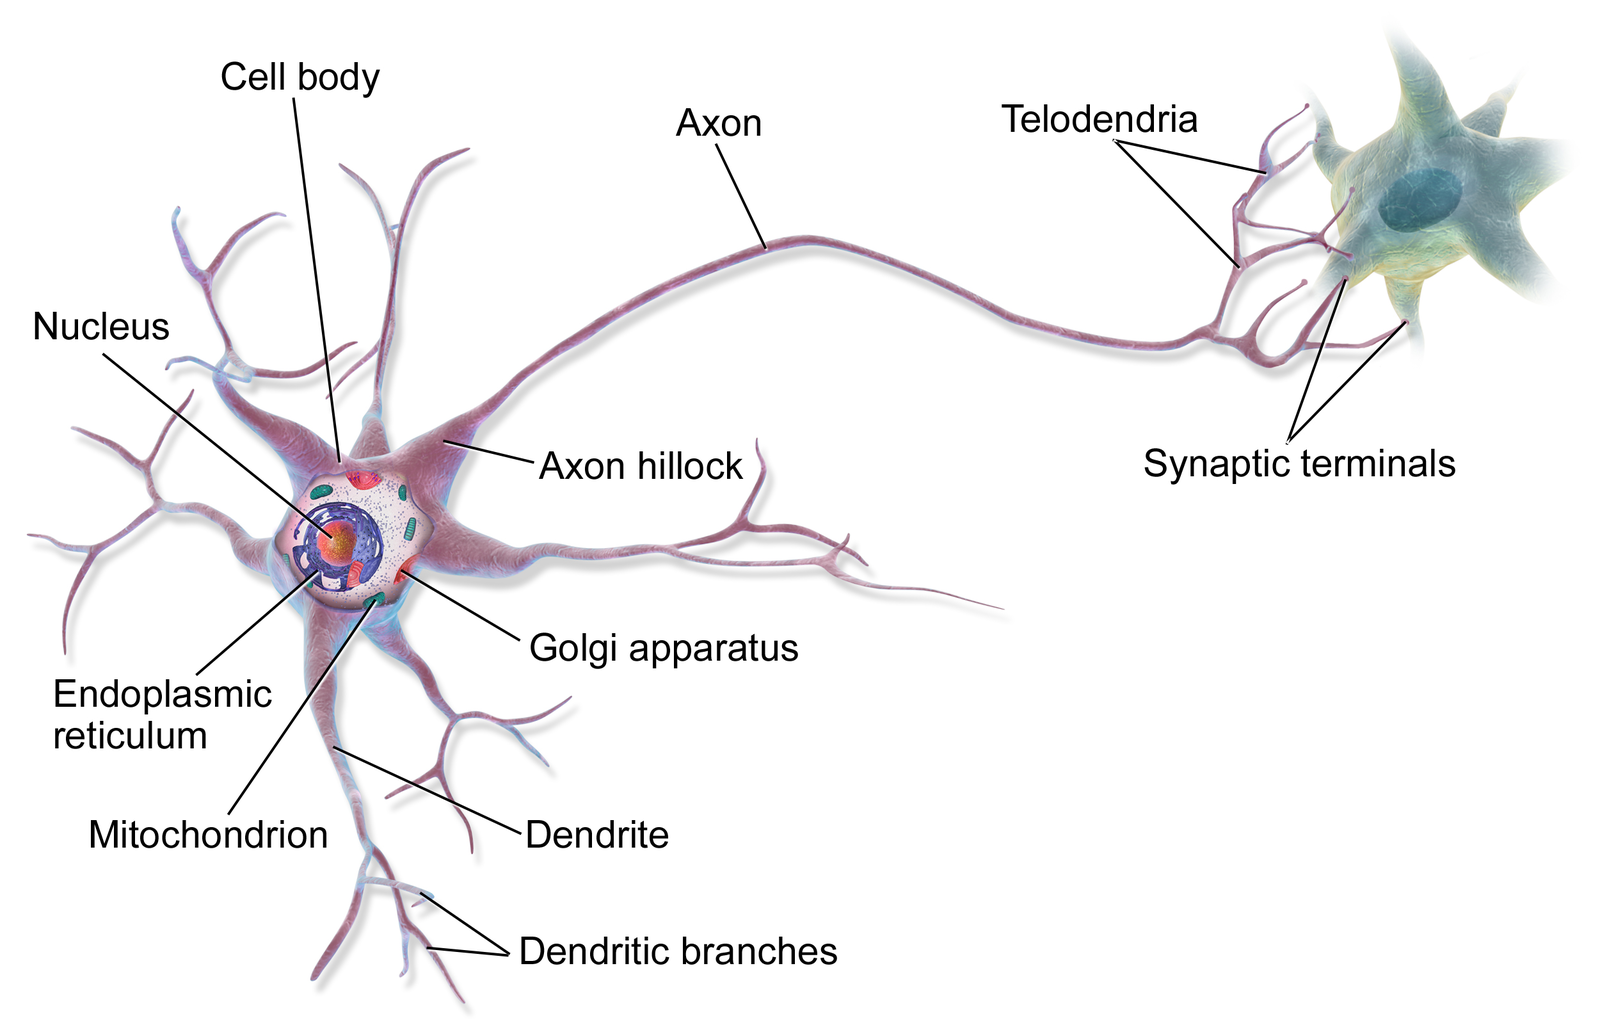
\includegraphics[width=\textwidth]{res/Blausen_MultipolarNeuron}
	\caption{Neural cell structure. Image by Bruce Blaus}
	\label{fig:Blausen-Neuron}
\end{figure}
There is however one behavior that until recently was believed to be specific to only neural cells
and even recent studies extend this ability to glial cells only.
This is ability to transfer a electric signal trough length of cell axon 

%----------------------------------------------------------------------------------------------------
\subsection{Cybernetics, first steps in modeling of neural systems}

%----------------------------------------------------------------------------------------------------
\subsection{Perceptron and first advent of neural networks}

%----------------------------------------------------------------------------------------------------
\subsection{Deep learning and second advent of neural networks}

%----------------------------------------------------------------------------------------------------
\subsection{Modern day}


%====================================================================================================
\section{Feed forward neural networks}

%----------------------------------------------------------------------------------------------------
\subsection{Mathematical model of neuron}
First mathematical model of the neural cell was created in 1943 by Warren MuCulloch and Walter Pitts.
It aimed at recreating an behavior of the neuron electric potenitial activation as a result of
synaptic potential reaching specific bias. What is important this model was never supposed to
precisely mimic behavior of biological neuron and as such do not include representation of metabolic
processes or even neurotransmition.
However despite significant simplification McCulloch-Pitts neuron proven to have many uses and
its basic structure were used to create most of modern day models.
Essentialy in this model neuron is a finction $f_n(x):\mathbb{R} \rightarrow \{ 0,1 \} $ where $n$
is size of input.
In such case equation describing neuron response is as follows:
The basic model of the neuron (neural layer) was created in 1943 by McCullough and Pitts 
\cite{McCulloch1943}. It described response of neural layer to multiple signals with
equation $y= \chi (W\cdot x+b)$, where $y$ is response, $x$ input, $W$ weights, $b$ bias and
$\chi$ is a step function.
Algorithm for automated adjustment of weights in relation to data was proposed in 1958
by Rosenblatt \cite{Rosenblatt58}. This model and all its successors can be described
as an aggregation, dampening, and activation signal path.
\begin{figure}[h] 
	\centering
	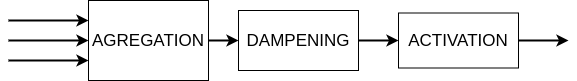
\includegraphics[width=10cm]{res/basic_neuron}
	\caption{Generalized model of a neuron}
	\label{fig:basic_neuron}
\end{figure}
In the case of McCullough-Pitts neuron aggregation is a weighted sum, dampening is the subtraction
of a bias and activation is a step function. While other models have some differences,
usually different activation functions, the basic signal flow remains unchanged.
While this model and its successors were inspired by a biological neuron there are much
more simplified. One of those simplifications is the lack of time-domain in the model which means
that response of a layer depends only on its current input.
This is in contrast with biological networks that are sensitive not only for a signal value
but also for its change over time.

%----------------------------------------------------------------------------------------------------
\subsection{Perceptron, abilities and limitations}
Simple perceptron is a McCullouch-Pitts neuron with a learnig alorithm assigned to it.
Therfore perceptron equation can be described as a :
\begin{equation}
	y = \chi (W\cdot x+b),
\end{equation}
where $\chi$ is a step function described as:
\begin{equation}
	\chi (x) =  
	\begin{cases}
		1       & \quad \text{if } u > 0\\
		0       & \quad \text{if } u \leq \\
	\end{cases}
\end{equation}
As perceptron rule is an example of a supervised learning it reqire a training set where for 
each input $x_{j}$ a corresponding expected output $d_{j}$ is provided. 
Then algorithm adjusts weights and bias of given neuron so that it response will 
correspond to expected one. 
Weights and biasa together are considered parameters of neuron and described as a:
\begin{equation}
	\phi = \{ W,b \}.
\end{equation}
\textbf{TODO: ADD A NEURON DIAGRAM}
Percetron rules works by excuting following steps:
\begin{itemize}
	\item If value of $y_{j}$ is equal to expected value $d_{j}$ then weights $W$ and 
		  bias $b$ remain unmodified.
	\item If value $y_{j}=0$ and $d_{j}=1$ then weights are to be updated acording to 
		  equation $W:=W+x_{j}$ and bias acording to equation $b:=b+1$.
	\item If value $y_{j}=1$ and $d_{j}=0$ then weights are to be updated acording to 
		  equation $W:=W-x_{j}$ and bias acording to equation $b:=b-1$.
\end{itemize}
After parameter update a new input-output pair is presented and algorithm repeats until all 
pairs from learning set are processed.
Perceptron rule was later generalied into a Widrow-Hoff rule according to which parameters are 
updated as described in equation :
\begin{equation}
	\Delta W_{j} = x_{j}(d_{j}-y_{j}),\\
	\Delta b_{j} = d_{j} - y_{j},\\
	W :=  W + \Delta W_{j},\\
	b := b + \Delta b_{j}.
\end{equation}
If only possible responses of neuron are 0 and 1 then Widrow-Hoff rule behaves exactly like a
perceptron rule.
Aim of lerning is minimalization of energy function of neuron response which is described as a:
\begin{equation}
	E = \sum_{j=0}^{n}(y_{j}-d_{j})^{2}
\end{equation}
Because step function is not continous in point 0 it is impossible to calculate it derivative
an therfore gradient based learing algorithms cannot be used for perceptron.
This limits this model to a single layer nework which is hightly problematic as such network
is very limited in its applications.
One of most basic examples ccan be a inability of perceptron to realize XOR function.
This is because in case of two dimensional input perceptron divides space into two lineary
seperable subspaces.
\textbf{TODO: IMAGE OF LOGIC FUNCTIONS}
Exculsive alternative do to its nature is not a lineary seperable function. It is however
possible to create a realization of XOR with perceptron like neurons by recreating a logic
circuit that is equivalent to XOR while using only OR, NOT, AND gates.
\textbf{TODO: IMAGE FROM LOGISIM CIRCUIT}

%----------------------------------------------------------------------------------------------------
\subsection{Multi layer neural networks}

%----------------------------------------------------------------------------------------------------
\subsection{Limitations on neural networks depth}


%====================================================================================================
\section{Recurrent networks and deep learning}

%----------------------------------------------------------------------------------------------------
\subsection{Deep learning models}

%----------------------------------------------------------------------------------------------------
\subsection{Simple recurrent networks}

%----------------------------------------------------------------------------------------------------
\subsection{Long short term memory networks}
Simple solution to problem of time independence is to concatenate response of neural layer
from previous cycle to it input $x'(t)=[x(t)|y(t-1)]$.
Such solution results in signal propagating trough time and influencing responses of future cycles,
if this is the only modification to the feed-forward model such layer is called Simple Recurrent
Unit (SRU).
\begin{figure}[h] 
	\centering
	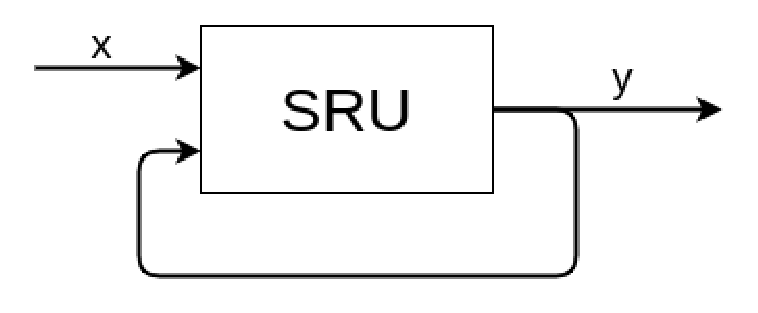
\includegraphics[width=5cm]{res/sru}
	\caption{Simple Reccurent Unit (SRU)}
	\label{fig:sru}
\end{figure}
While this solution makes model time aware it has its own problems, mainly a signal vanishing
issue. Since the input signal from a cycle, $n$ has direct influence only on a response of this
cycle and for each subsequent cycle, it is the only through a feedback loop.
Influence of input $n$ on response of cycle $n+k$ grows inverse proportional to $k$.
This means that in this model only those regularities that appear over short time periods can
be detected.
Making weights on feedback bigger will not eliminate the problem and instead replace it with signal
an explosion that causes a response to reach maximum value if a strong signal appeared on input at
least once.
One of the possible solutions to this issue is the addition of long term memory which will regulate
forward and loopback path influence on neuron response, such a solution is used in long short
term memory (LSTM) networks \cite{Hochreiter1997}.
% TODO: Move legend below, write more precisely about neuron and no neurn
\begin{figure}[h] 
	\centering
	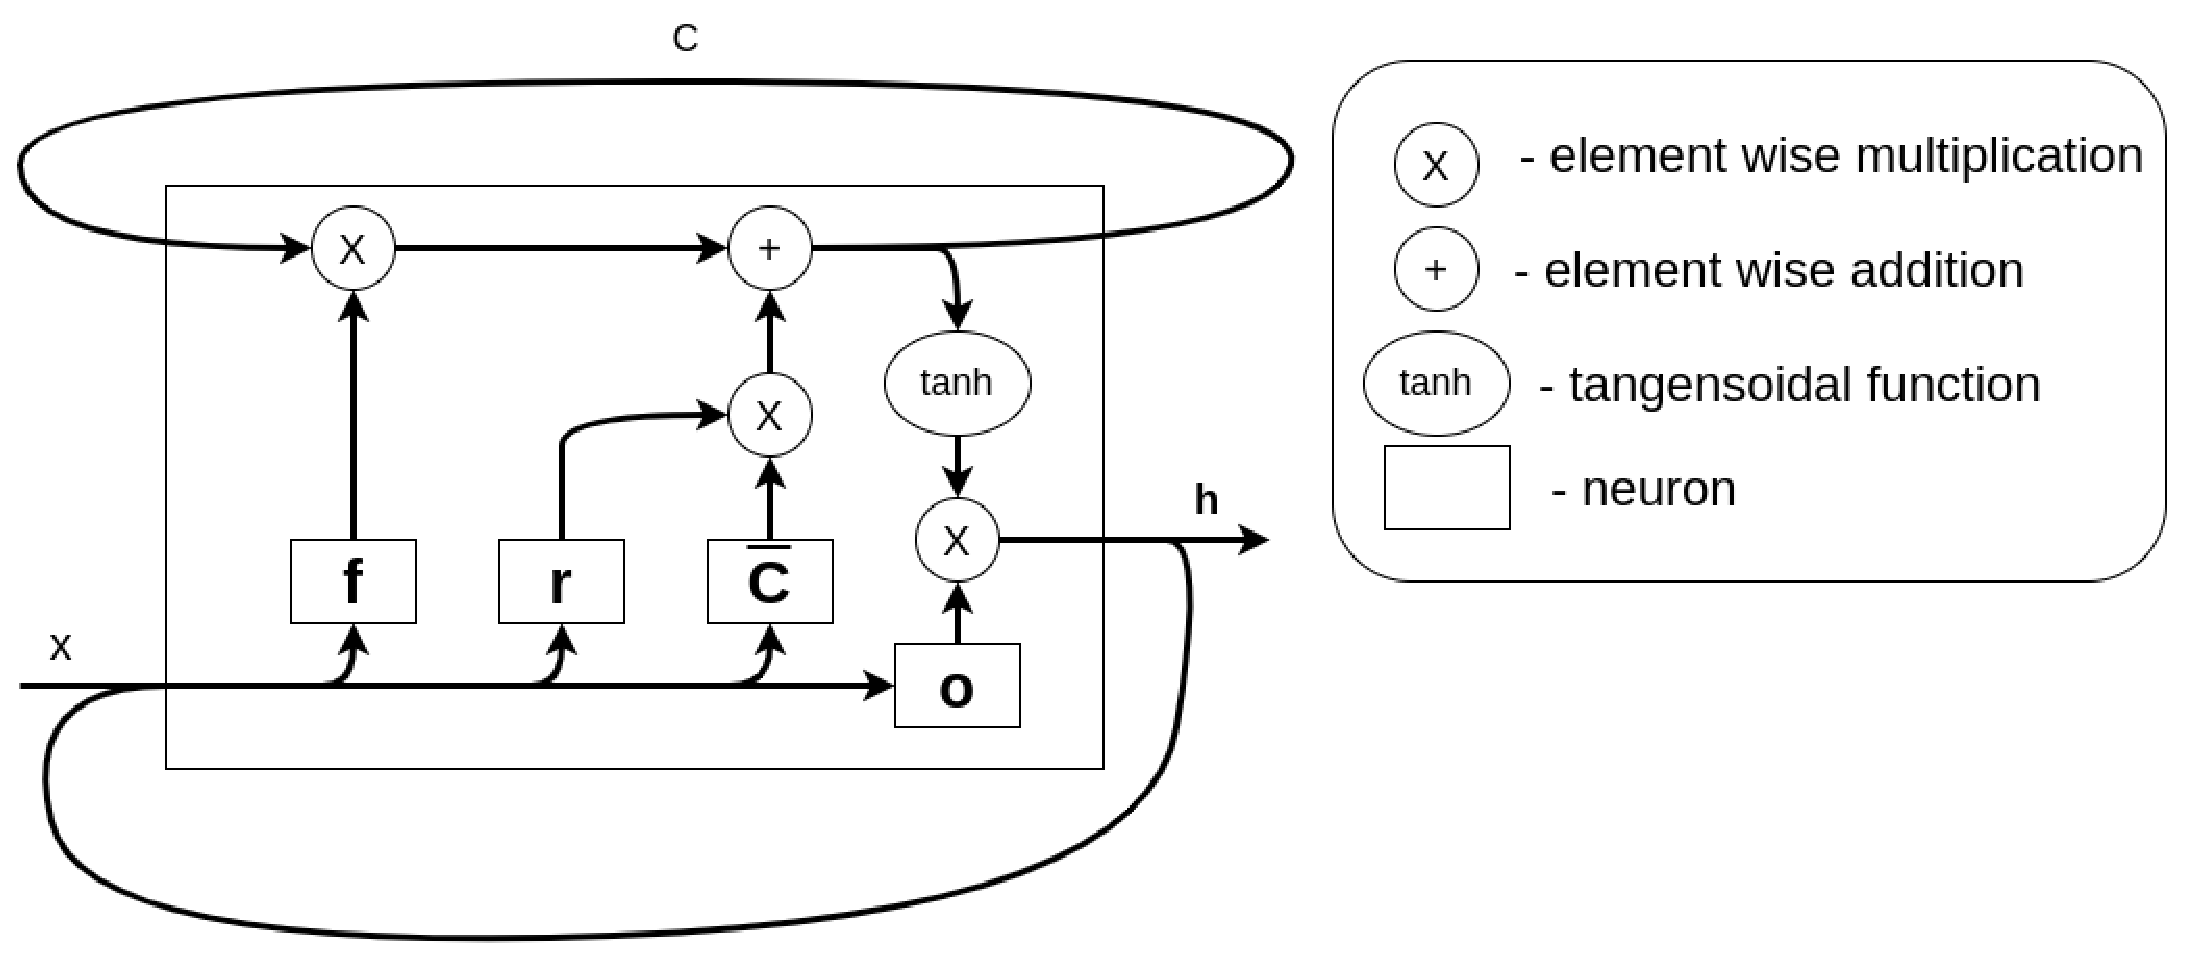
\includegraphics[width=10cm]{res/lstm}
	\caption{LSTM layer}
	\label{fig:lstm}
\end{figure}
Single LSTM neuron consists of four basic neurons and two non-neuron operations:
\begin{itemize}
	\item $x'(t)=[x(t)|h(t-1)]$,
	\item $o_t=\sigma (W_o x'_t+b_o)$,
	\item $r_t=\sigma (W_r x'_t+b_r)$,
	\item $f_t=\sigma (W_f x'_t+b_f)$,
	\item $\bar{C}_t=\tanh (W_c x'_t+b_c)$,
	\item $C_t=f_t\odot C_{t-1}+r_t\odot \bar{C}_t$,
	\item $h_t=o_t\odot \tanh (C_t)$,
\end{itemize}
with $W$ and $b$ being weights and biases for each basic neuron, $x$ input, $y$ output and
$C$ long term memory. As can be seen, $o_t$ is the equivalent of SRU and is moderated by
long term memory before propagating as output. Temporary value of long term memory based
only on current output $\bar{C}_t$ is calculated and then with help of neurons $r$ and $f$
is transformed into its final value.
Neuron $r$ is called remembering gate and influences to what degree temporary long term
a memory from a given cycle affects its final value while $f$ is forgetting gate and
decides the influence of long-term memory from the last cycle on the current one.
Thanks to such implementation our model can learn to detect both long term regularities and 
short term ones.

